% task4.tex — Unsupervised Anomaly Detection and Interpretation

\section{UNSUPERVISED ANOMALY DETECTION AND INTERPRETATION} \label{sec:task4}

This section explores purely unsupervised clustering approaches (K-Means and DBSCAN) for anomaly detection, evaluating their ability to separate attack types without label supervision.

% --- K-Means ---
\subsection{K-Means Clustering} \label{sec:kmeans}

    We applied K-Means with $k = 4$ clusters on the full training set. 
    Following the assignment assumptions, we presume that a domain expert may know the approximate number of common traffic categories, but lacks access to the specific attack labels associated with individual samples.
    The resulting clusters were therefore generated in a completely unsupervised manner and evaluated afterwards using the ground-truth labels.

    \begin{table}[H]
        \centering
        \begin{tabular}{@{}crcccl@{}}
            \toprule
            \textbf{Cluster} & \textbf{Size} & \textbf{Silhouette} & \textbf{Dominant Class} & \textbf{Purity} & \textbf{Composition} \\
            \midrule
            0 & 1,560  & 0.261 & probe (54\%)   & Mixed & probe 54\%, normal 28\%, dos 18\% \\
            1 & 1,422  & 0.753 & dos (100\%)    & Pure  & dos 100\% \\
            2 & 9      & 0.392 & normal (100\%) & Pure  & normal 100\% \\
            3 & 12,072 & 0.461 & normal (85\%)  & Mixed & normal 85\%, probe 8\%, dos 6\%, r2l 1\% \\
            \bottomrule
        \end{tabular}
        \vspace{0.5em}
        \caption{K-Means cluster composition and quality ($k = 4$, training set).}
        \label{tab:kmeans_clusters}
    \end{table}

    \vspace{-0.3cm}

    \noindent
    The average silhouette score of 0.468 indicates moderate cluster separation overall.
    \textbf{Cluster~1} exhibits a high silhouette score of 0.753 because DoS floods generate a distinctly dense region in feature space, driven by high SYN error rates and connection counts.
    \textbf{Cluster~0} has the lowest silhouette (0.261), corresponding to an ambiguous boundary region that mixes probe, normal, and some DoS traffic.
    Conversely, the algorithm struggled heavily with stealthy attacks: almost all 145 R2L attacks were absorbed into the massive, normal-dominated \textbf{Cluster~3}. 
    This suggests that R2L attacks share many mathematical characteristics with normal traffic under the chosen feature representation and distance assumptions, preventing a variance-minimizing algorithm like K-Means from partitioning them effectively.

    \textbf{Cluster~2} contains only 9 samples, all labelled as normal traffic. 
    Although very small, this cluster is still informative because it identifies a group of highly atypical normal observations that are separated from the rest of the dataset. 
    Such clusters are particularly relevant for the subsequent DBSCAN analysis, where pure-normal clusters can be used to estimate density parameters.

    \begin{figure}[H]
        \centering
        \begin{minipage}{0.53\linewidth}
            \centering
            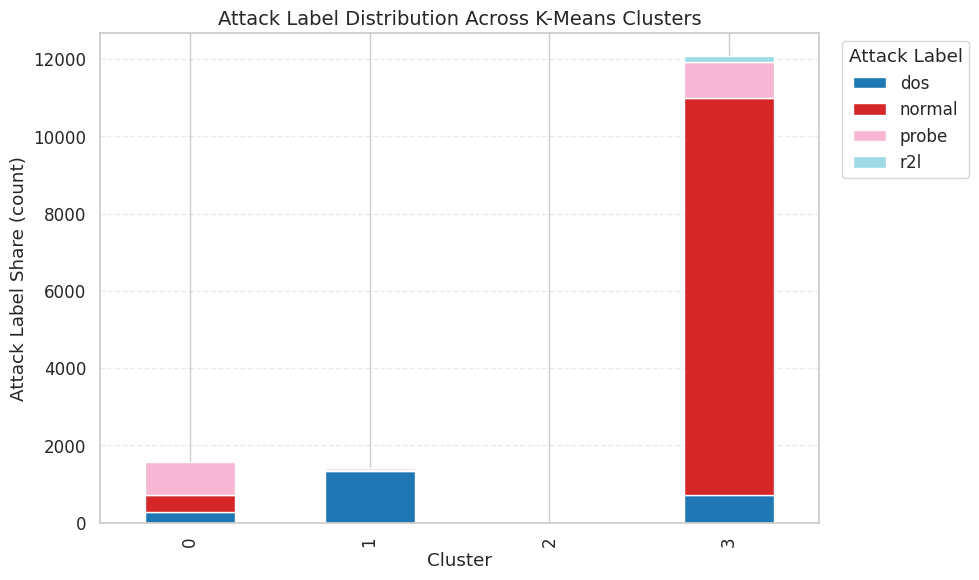
\includegraphics[width=\linewidth]{images/task4/task4_kmeans_attack_distribution.png}
            \caption{K-Means ($k = 4$) cluster composition by traffic type.}
            \label{fig:kmeans_attack_dist}
        \end{minipage}\hfill
        \begin{minipage}{0.45\linewidth}
            \centering
            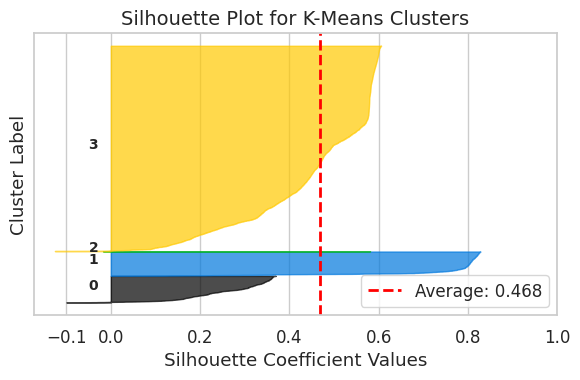
\includegraphics[width=\linewidth]{images/task4/task4_kmeans_silhouette.png}
            \caption{K-Means ($k = 4$) silhouette coefficient distribution.}
            \label{fig:kmeans_silhouette}
        \end{minipage}
    \end{figure}

    \noindent
    Using majority voting to assign binary labels to clusters, K-Means achieves a training F1-Macro of \textbf{0.7954}.
    However, this post-hoc labelling requires access to ground-truth labels for evaluation and does not generalize to unseen data, limiting its practical utility as a standalone IDS.

% --- t-SNE ---
\subsection{t-SNE Visualization} \label{sec:tsne}

    We applied t-SNE to project the training data into 2D, testing perplexity values of 5 (local focus), 30 (balanced), and 100 (global).
    \textbf{Perplexity = 30} provides the best balance between local and global structure, preserving meaningful class separability without over-fragmenting the data.

    \begin{figure}[H]
        \centering
        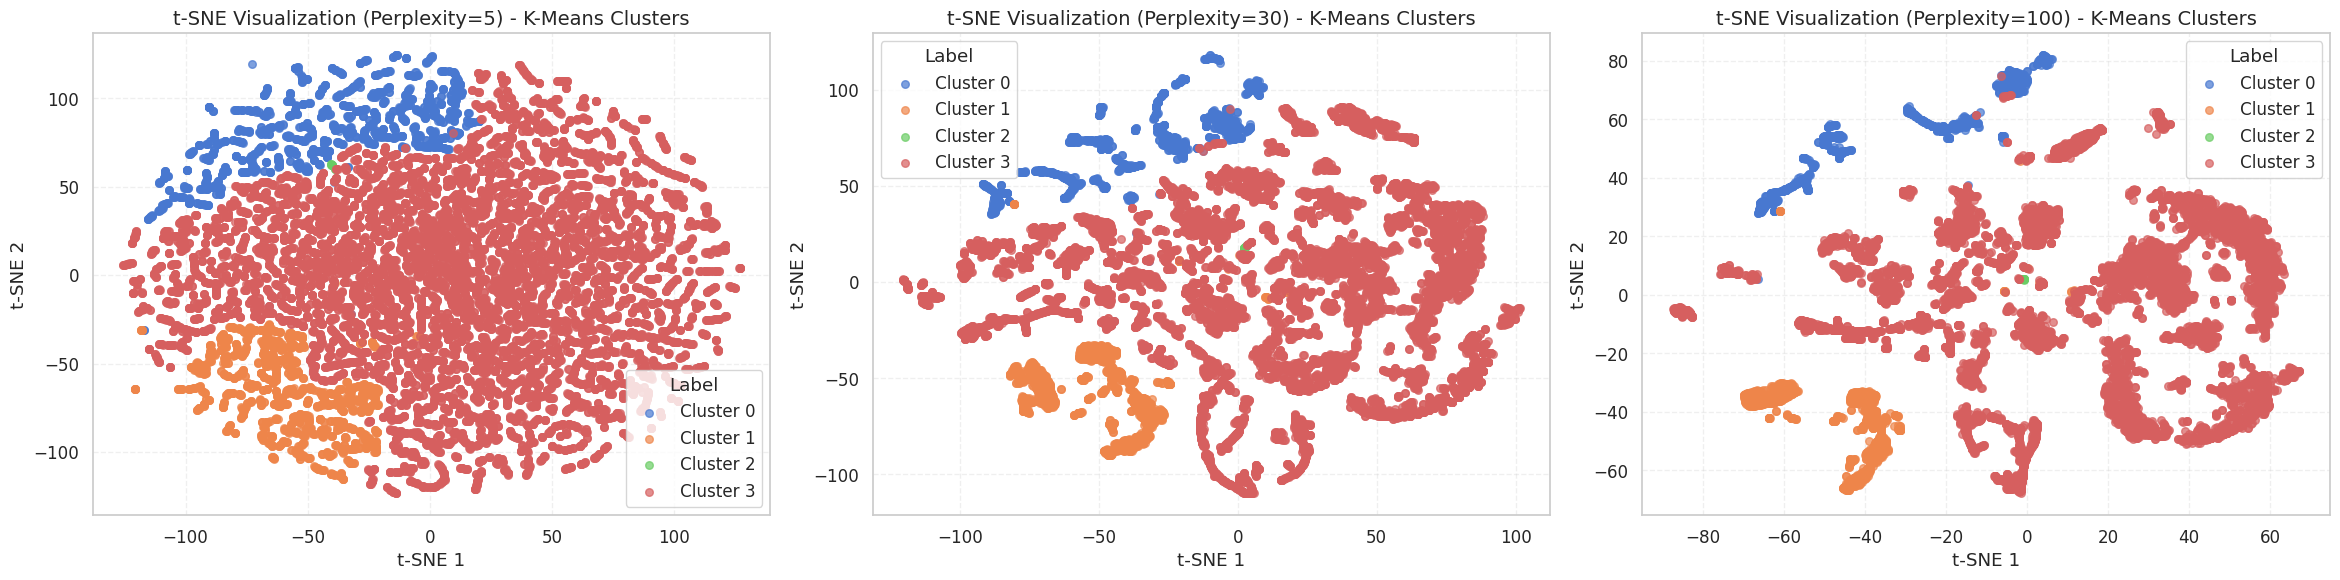
\includegraphics[width=\linewidth]{images/task4/task4_tsne_perplexity_comparison.png}
        \caption{t-SNE at three perplexity values. Perplexity = 5 over-fragments the data into micro-clusters; perplexity = 100 merges distinct attack islands; perplexity = 30 preserves both local separation and global structure.}
        \label{fig:task4_tsne_perplexity}
    \end{figure}

    \noindent
    The side-by-side comparison in \Cref{fig:task4_tsne} reveals that K-Means quite well separates the DoS cluster (Cluster~1 aligns cleanly with the DoS island in t-SNE space), but \textbf{Cluster~3 absorbs diverse traffic types}.
    Most notably, R2L samples appear largely embedded within regions dominated by normal traffic in the t-SNE projection, providing a visual explanation for the difficulty encountered by K-Means when attempting to isolate them.

    \begin{figure}[H]
        \centering
        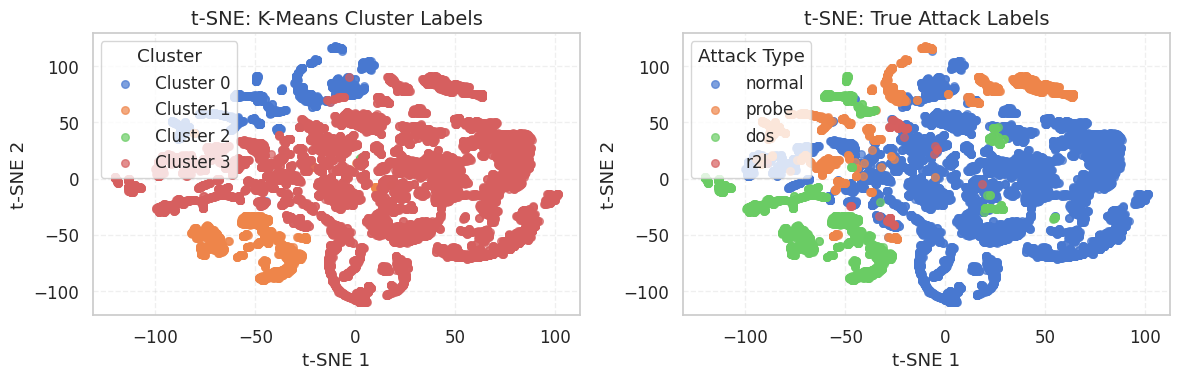
\includegraphics[width=\linewidth]{images/task4/task4_tsne_comparison.png}
        \caption{t-SNE (perplexity = 30). Cluster~1 aligns cleanly with DoS (bottom-left), but Cluster~3 absorbs both probe and R2L traffic.}
        \label{fig:task4_tsne}
    \end{figure}

% --- DBSCAN ---
\subsection{DBSCAN Clustering} \label{sec:dbscan}

    DBSCAN identifies dense clusters and labels the remaining points as noise ($-1$), which we interpret as potential anomalies. 
    We utilized Cosine distance throughout this clustering analysis to emphasize similarities in traffic profiles rather than absolute traffic volume, which can vary substantially across connections. 
    This directional alignment provides a alternative neighborhood definition for DBSCAN than raw magnitude differences.

    Following the assignment guidelines, we first inspected the K-Means solutions across various parameter configurations to identify the smallest cluster composed exclusively of benign traffic samples. 
    This optimization heuristic yielded a baseline target value of $\texttt{min\_pts}=7$ (derived from Cluster~2 in \Cref{tab:kmeans_clusters}). 
    However, such a small value is likely to generate clusters around very small groups of observations, including isolated normal outliers. 
    To investigate more robust and conservative density definitions, we extended our exploratory parameter sweep to include $\texttt{min\_pts} \in \{7, 100, 500, 1600\}$. 
    For each setting, the corresponding operational $\epsilon$ was determined using the sorted $k$-distance graph elbow rule, locating the inflection point at the 70th percentile of sorted distances (yielding $\epsilon = 0.635$ for $\texttt{min\_pts}=1600$, and $\epsilon = 0.260$ for $\texttt{min\_pts}=500$).

    % \begin{figure}[H]
    %     \centering
    %     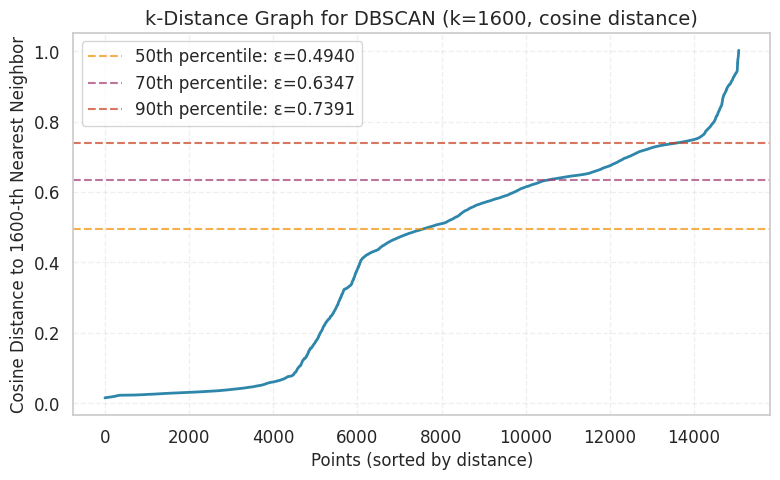
\includegraphics[width=0.6\linewidth]{images/task4/task4_dbscan_kdistance_minpts1600.png}
    %     \caption{$k$-distance graph for $\texttt{min\_pts} = 1600$ (cosine dist). The elbow (70th percentile) of the sorted distances yields $\epsilon = 0.635$.}
    %     \label{fig:task4_dbscan_kdistance}
    % \end{figure}

    \noindent
    % The macro-behavior of the DBSCAN algorithm transforms substantially as the structural density threshold increases. 
    The behavior of DBSCAN changes considerably as the density threshold increases.
    Lower values of $\texttt{min\_pts}$ generate a highly fragmented space with numerous micro-clusters, classifying a significant volume of sparse, legitimate observations as noise. 
    Conversely, elevated parameters progressively force the data coordinates to coalesce into massive, overarching spatial domains.

    Among the explored configurations within our parameter sweep, $\texttt{min\_pts}=500$ ($\epsilon = 0.260$) provides the most balanced and interpretable trade-off between cluster granularity and noise isolation. 
    This specific configuration populates exactly four distinct data clusters and captures the highest overall quantitative metric with a training F1-Macro score of $0.4874$. 
    Although the resulting noise fraction remains heavily dominated by benign traffic anomalies (70.7\%), it provides the most interpretable compromise between cluster granularity and noise detection among the tested configurations.

    \begin{table}[H]
        \centering
        \begin{tabular}{@{}rcccccc@{}}
            \toprule
            \textbf{min\_pts} & \textbf{$\epsilon$} & \textbf{Clusters} & \textbf{Noise \%} & \textbf{F1-Macro} & \textbf{Noise: Normal} & \textbf{Noise: Anomaly} \\
            \midrule
            7    & 0.064 & 40 & 3.2\%  & 0.4285 & 80.9\% & 19.1\% \\
            100  & 0.053 & 17 & 21.8\% & 0.4707 & 76.0\% & 24.0\% \\
            500  & 0.260 & 4  & 14.2\% & 0.4874 & 70.7\% & 29.3\% \\
            1600 & 0.635 & 1  & 2.0\%  & 0.4466 & 52.5\% & 47.5\% \\
            \bottomrule
        \end{tabular}
        \vspace{0.5em}
        \caption{DBSCAN results for different values of $\texttt{min\_pts}$.}
        \label{tab:dbscan_comparison}
    \end{table}

    \vspace{-0.3cm}

    \noindent
    Adjusting the density parameter up to $\texttt{min\_pts}=1600$ changes the noise cluster's composition, moving it closer to an even split with malicious instances (47.5\% true anomalies). 
    However, this marginal shift comes at a critical structural cost, collapsing almost the entire feature space into a single massive cluster (Cluster~0), as detailed in \Cref{tab:dbscan_clusters}.

    \begin{table}[H]
        \centering
        \begin{tabular}{@{}lccc@{}}
            \toprule
            \textbf{Attack Label} & \textbf{Noise ($-1$)} & \textbf{Cluster 0} & \textbf{Total} \\
            \midrule
            Normal & 159 & 10,599 & 10,758 \\
            DoS    & 138 & 2,192  & 2,330  \\
            Probe  & 1   & 1,829  & 1,830  \\
            R2L    & 5   & 140    & 145    \\
            \midrule
            Total  & 303 & 14,760 & 15,063 \\
            \bottomrule
        \end{tabular}
        \vspace{0.5em}
        \caption{DBSCAN matrix breakdown under a single-cluster collapse ($\texttt{min\_pts} = 1600$, $\epsilon = 0.635$).}
        \label{tab:dbscan_clusters}
    \end{table}
    
    \vspace{-0.3cm}

    % \noindent
    % For this dataset, the empirical density profile mapped by DBSCAN does not align cleanly with the semantic dichotomy separating normal connections from malicious network anomalies. 
    % This structural limitation manifests across three specific profiles:
    % \begin{itemize}
    %     \item \textbf{DoS Floods:} Volumetric flood attacks launch thousands of rapid, structurally identical connection packets. 
    %         DBSCAN naturally identifies this intense concentration as a high-density, valid cluster core, allowing it to bypass the noise-based detector completely.
    %     \item \textbf{Sparse Normal Outliers:} Completely benign connections exhibiting atypical session durations or invoking rarely utilized services appear spatially isolated within the high-dimensional space, causing the model to incorrectly flag them as malicious noise.
    %     \item \textbf{R2L Intrusions:} Sneakier, low-volume privilege-escalation exploits closely mirror normal traffic behavior, remaining embedded within normal-dominated clusters across all evaluated configurations.
    % \end{itemize}
    % 
    % Overall, these results suggest that density-based clustering alone is insufficient to accurately separate normal and anomalous traffic in this setting. 
    % While DBSCAN provides exceptional insights into the structural topology of the network data, it does not constitute a viable standalone intrusion detection system.

    \noindent
    For this dataset, the density structure mapped by DBSCAN does not align cleanly with the actual distinction between normal and malicious traffic. 
    This limitation manifests in three main ways:
    \begin{itemize}
        \item \textbf{DoS Floods:} Because volumetric flood attacks consist of thousands of identical, rapid packets, DBSCAN groups them into a dense cluster rather than identifying them as noise anomalies.
        \item \textbf{Sparse Normal Outliers:} Atypical but benign connections (e.g., with unusual session durations or rare services) appear isolated and are falsely flagged as malicious noise.
        \item \textbf{R2L Intrusions:} Low-volume privilege-escalation exploits closely mimic normal behavior, remaining hidden inside normal clusters.
    \end{itemize}

    \noindent
    Overall, these results show that density-based clustering alone cannot reliably separate normal and anomalous traffic here. 
    While DBSCAN helps analyze the structure of the network data, it is not suitable as a standalone intrusion detection system.
